\documentclass[11pt,a4paper]{article}
\usepackage[margin=18mm,top=16mm,bottom=16mm]{geometry}
\usepackage{fontspec}
\IfFontExistsTF{Times New Roman}{\setmainfont{Times New Roman}}{\setmainfont{TeX Gyre Termes}}
\usepackage{amsmath,booktabs,caption,titlesec,graphicx}
\usepackage[unicode,hidelinks]{hyperref}
\hypersetup{pdftitle={Thăm dò CLIP: rà soát nhãn và kiểm chứng quan hệ trên tập ảnh mới}}
\renewcommand{\tablename}{Bảng}\renewcommand{\figurename}{Hình}\renewcommand{\refname}{Tài liệu tham khảo}
\titleformat{\section}{\normalsize\bfseries}{\thesection.}{0.5em}{}
\titlespacing*{\section}{0pt}{7pt}{3pt}
\captionsetup{font=small,labelfont=bf,skip=4pt}
\setlength{\parindent}{0pt}\setlength{\parskip}{4pt}\setlength{\tabcolsep}{5pt}
\renewcommand{\arraystretch}{1.1}\hyphenpenalty=10000\emergencystretch=2em
\newcommand{\NewAcc}{53,00}
\newcommand{\NewCI}{[43,29; 62,49]}
\newcommand{\NewP}{0,3086}
\newcommand{\NewCorrect}{53}
\newcommand{\NewBoth}{4,00}
\newcommand{\NewTwoWay}{51,50}
\newcommand{\OldCleanAcc}{28,41}
\newcommand{\OldCleanCI}{[22,16; 35,23]}
\newcommand{\OldCleanHorizontal}{93}
\newcommand{\OldCleanPair}{55,91}
\newcommand{\DeltaAcc}{-1,00}
\newcommand{\DeltaCI}{[-15,00; 12,00]}
\newcommand{\NearTies}{0}
\newcommand{\ExactTies}{0}

\begin{document}
\begin{center}
{\large\bfseries BÁO CÁO TIẾN ĐỘ — ĐỀ TÀI 14}\\[3pt]
{\Large\bfseries Thăm dò CLIP: rà soát nhãn và kiểm chứng\\ quan hệ không gian trên tập ảnh mới}\\[4pt]
{\small Computer Vision \quad|\quad Cập nhật: 04/11/2026}
\end{center}
\textbf{Tóm tắt.} Nghiên cứu giữ cố định CLIP ViT-B/32, tiếp nối năm baseline và các phép thăm dò có đối chứng. Sau tự rà soát nhãn, 176/200 ảnh tự nhiên cũ được giữ; accuracy bốn lựa chọn thay đổi từ 28,00\% thành \OldCleanAcc\%. Phép ghép hai ảnh với hai caption được chốt trước và kiểm chứng trên 100 nguồn ảnh mới, không trùng bất kỳ ảnh nào trong 400 ứng viên từng xem. Kết quả ghép đúng \NewAcc\%, CI Wilson 95\% \NewCI\%, kiểm định nhị thức một phía $p=\NewP$; chưa có bằng chứng rõ về xác suất ghép đúng cao hơn 50\%. Chỉ \NewBoth\% cặp có cả hai ảnh được dự đoán đúng riêng rẽ. Kết quả bổ sung bằng chứng về hành vi thiếu nhất quán; không chứng minh mô hình hoàn toàn không chứa thông tin vị trí.

\section{Phạm vi và kết quả nền}
Sử dụng duy nhất OpenAI CLIP ViT-B/32~\cite{clip}, giữ trọng số, preprocessing, FP32/QuickGELU và batch 32; không fine-tuning. Môi trường conda gen, GPU RTX 4050 Laptop. Dự đoán bằng cosine của vector ảnh và caption chuẩn hóa. Năm test baseline trên 46.948 ảnh đạt: CIFAR-100 64,48\%; Flowers102 63,77\%; Oxford-IIIT Pet 85,06\%; DTD partition 1 42,45\%; Food-101 82,31\%.

Phần đào sâu trước đây gồm 1.440 ảnh hình học/8.640 phép thử: nhận dạng đối chứng 96,94\%, nhưng quan hệ chỉ 27,36\%; cặp trái/phải cùng đúng 0,56\%, không nhóm nào đúng cả bốn vị trí. Hai cách viết tương đương T0 chỉ cùng dự đoán ở 16,25\% ảnh. Các tỷ lệ này thể hiện khoảng cách giữa nhận dạng thuộc tính và kết hợp quan hệ trong bộ kiểm tra.

Trên CIFAR-100, category đúng đạt 62,92\%, thấp hơn baseline 1,56 điểm \% (CI [−2,14; −0,98]); trung tính đạt 64,09\%, trung bình năm category sai đạt 54,19\%. Điểm lớp đúng tăng trung bình 0,001628 nhưng đối thủ mạnh nhất tăng 0,002908, làm margin giảm 0,001280. Lỗi trong và ngoài nhóm đều tăng. Category đúng tốt hơn category sai, nhưng không mặc nhiên cải thiện baseline theo cách viết đang xét.

\section{Tự rà soát nhãn và phân tích độ nhạy trên tập cũ}
Trợ lý xem lại đủ 200 ảnh đã chọn từ COCO val2014~\cite{coco}, không hiển thị scores/dự đoán từng ảnh hoặc lý do chấp nhận cũ. Kết quả tổng hợp đã biết; đây là \textbf{tự rà soát}, không phải annotator độc lập hoặc mù hoàn toàn. Tiêu chí kiểm tra: nhận ra hai vật thể, tên lớp phù hợp, quan hệ rõ và vật thể còn nhìn thấy trong center crop. Không sửa các artifact cũ.

Có 24 ảnh bị loại khỏi phân tích độ nhạy vì che khuất/cắt xén, tên lớp mơ hồ hoặc mục tiêu là hình in trên bao bì. Giữ 176 ảnh; accuracy T2 thuận trên bốn lựa chọn là \OldCleanAcc\%, CI bootstrap \OldCleanCI\%, so với 28,00\% trước đó. Phần quan hệ ngang còn \OldCleanHorizontal\ nguồn; ghép đúng 52/93, tức \OldCleanPair\%, so với 54/100 ban đầu. Điểm ước lượng thay đổi nhỏ, nhưng không phải kiểm định tương đương; bộ 176 ảnh không còn cân bằng hoàn toàn bốn nhãn. Tự rà soát vẫn chủ quan, không chứng minh mọi annotation bị loại đều sai.

\section{Giao thức kiểm chứng được định trước}
Giả thuyết phát sinh từ phân tích ghép cặp hậu nghiệm cũ; giao thức xác nhận được ghi trước lựa chọn cuối và suy luận mới. Loại toàn bộ 400 source ID đã từng xem, giữ nguyên ngưỡng hình học, chỉ xét trái/phải để mirror tạo phản thực thật sự. Còn 178 ứng viên mới; rà soát toàn bộ, nhận 112 và chọn 100 ảnh đầu theo thứ tự SHA256 với seed 14031. Sàng lọc dHash crop và mirror không phát hiện cặp dưới ngưỡng ≤6; trực quan loại thêm một cảnh gần trùng cũ. Danh sách đóng băng lúc 16:17:49 UTC, trước khi run bắt đầu 16:19:04 UTC, ngày 04/11/2026.

\newpage
Mỗi nguồn có ảnh gốc và bản lật: 200 ảnh đầu vào, ba template × hai thứ tự, tổng 1.200 lượt chấm caption. T2 thuận ``an image of A r B'' là điều kiện chính; T0 ``a photo of A r B'', T1 ``A is r B'' và thứ tự đảo tương đương là phụ. Không chọn template tốt nhất từ kết quả. Smoke và kiểm chứng phép tính dùng scores cũ, không mở một phần tập mới để điều chỉnh.

Với hai ảnh sắp theo nhãn trái/phải và hai caption tương ứng, ma trận cosine $S$ cho
\[
D=S_{11}+S_{22}-S_{12}-S_{21}.
\]
$D>0$ được tính ghép đúng; D=0 tính sai và báo riêng near-tie $|D|\leq10^{-6}$. Thành phần cộng riêng theo ảnh hoặc caption triệt tiêu trong hiệu này; không loại mọi thiên lệch. Thiết kế ghép ảnh--text tham khảo hướng đánh giá tính kết hợp~\cite{winoground}, không tái lập Winoground.

Metric chính là accuracy ghép cặp, CI Wilson 95\%, bootstrap 2.000 lần theo nguồn ảnh (seed 14031), và kiểm định nhị thức một phía $H_0:p\leq0,5$, $H_1:p>0,5$, $\alpha=0,05$. Mỗi nguồn là một đơn vị, không coi bản lật/caption là mẫu độc lập. Tập mới chỉ có nhãn ngang nên không so accuracy bốn lựa chọn của nó với 28\% trên bốn quan hệ cân bằng cũ.

\section{Kết quả kiểm chứng}
\begin{center}
\captionof{table}{Ghép cặp T2 thuận. Cột cuối yêu cầu model chọn đúng caption cho từng ảnh trong cả hai ảnh; khác với chọn cách ghép toàn cặp.}
\small\begin{tabular}{@{}lrrrr@{}}
\toprule
Tập ảnh ngang & Số cặp & Ghép đúng (\%) & CI Wilson 95\% & Cả hai ảnh đúng (\%) \\
\midrule
Cũ, đầy đủ & 100 & 54,00 & [44,26; 63,44] & 4,00 \\
Cũ, sau tự rà soát & 93 & 55,91 & [45,79; 65,57] & 4,30 \\
Mới, xác nhận & 100 & 53,00 & [43,29; 62,49] & 4,00 \\
\bottomrule
\end{tabular}

\end{center}
\vspace{-4pt}
Kết quả chính mới là \textbf{\NewCorrect/100 = \NewAcc\%}, CI Wilson \NewCI\%, CI bootstrap [43,00; 63,00]\%. Với $p=\NewP$, không bác bỏ $H_0$: chưa có bằng chứng rõ rằng xác suất ghép đúng vượt 50\%. Không suy ra p đúng bằng 50\%, không có thông tin vị trí, hoặc model tương đương đoán ngẫu nhiên. Có \ExactTies\ exact tie và \NearTies\ near-tie ở điều kiện chính.

Phân loại trái/phải từng ảnh đạt \NewTwoWay\%, nhưng cả ảnh gốc và mirror cùng đúng chỉ \textbf{\NewBoth\%}. Một caption có thể thắng trên cả hai ảnh dù hiệu tổng điểm ghép mang dấu đúng; vì vậy accuracy ghép cặp và tính đúng đồng thời đo hai khía cạnh khác nhau. So với 54\% cũ, chênh lệch mới−cũ là \DeltaAcc\ điểm \%, CI bootstrap hai tập độc lập \DeltaCI. Khoảng rộng, chưa cho phép kết luận hai tập tương đương hoặc tập mới kém hơn. Không gộp dữ liệu thăm dò vào kết quả xác nhận chính.

\begin{center}
\captionof{table}{Đủ sáu điều kiện trên 100 nguồn mới. Chỉ T2 thuận là phép kiểm định chính; các điều kiện khác mang tính mô tả.}
\small\begin{tabular}{@{}lrrrr@{}}
\toprule
Điều kiện mới & Đúng/tổng & Ghép đúng (\%) & CI Wilson 95\% & Cả hai ảnh đúng (\%) \\
\midrule
T0 / thuận & 52/100 & 52,00 & [42,32; 61,54] & 3,00 \\
T0 / đảo tương đương & 54/100 & 54,00 & [44,26; 63,44] & 4,00 \\
T1 / thuận & 55/100 & 55,00 & [45,24; 64,39] & 2,00 \\
T1 / đảo tương đương & 54/100 & 54,00 & [44,26; 63,44] & 1,00 \\
T2 / thuận & 53/100 & 53,00 & [43,29; 62,49] & 4,00 \\
T2 / đảo tương đương & 50/100 & 50,00 & [40,38; 59,62] & 3,00 \\
\bottomrule
\end{tabular}

\end{center}
\vspace{-4pt}
Các điểm ghép đúng phụ nằm trong khoảng 50--55\%, tỷ lệ cả hai ảnh đúng 1--4\%. Công bố cả kết quả này giúp tránh lựa chọn thuận lợi một cách viết sau khi xem test. Không thực hiện điều chỉnh prompt hoặc huấn luyện từ kết quả mới.

\newpage
\begin{center}
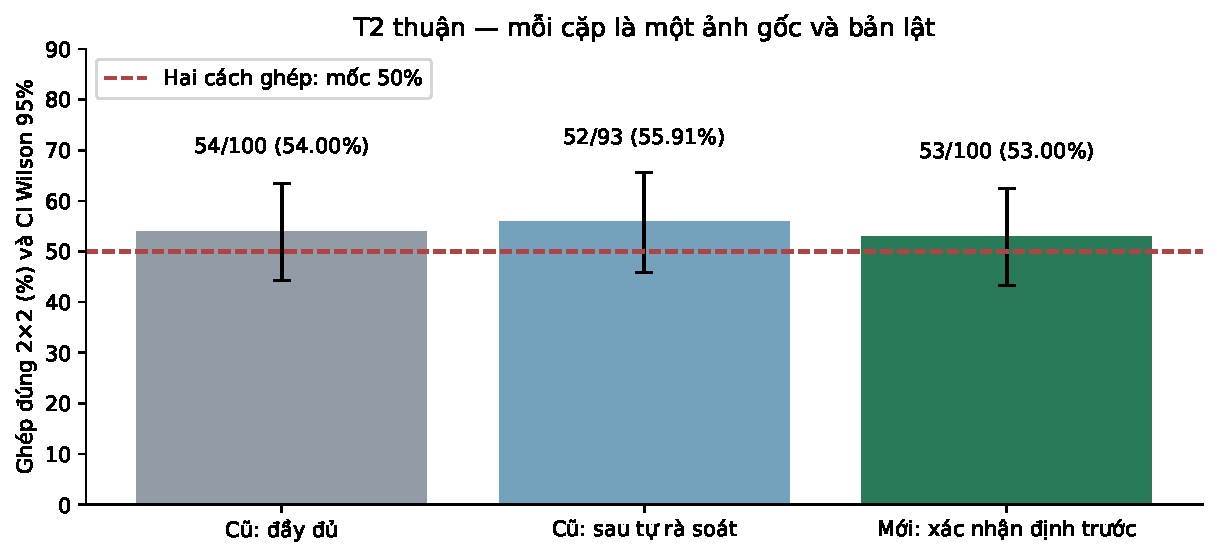
\includegraphics[width=0.80\linewidth]{confirmation.pdf}
\captionof{figure}{Accuracy ghép cặp chính và CI Wilson 95\%. Hai cột đầu dùng lại dữ liệu cũ; cột cuối là tập xác nhận mới. Không coi ba cột là ba tập độc lập.}
\end{center}
\section{Diễn giải đóng góp và giới hạn}
Chuỗi bằng chứng hiện tại gồm: nhận dạng thuộc tính hình học tốt nhưng quan hệ thiếu nhất quán; category làm thay đổi cạnh tranh giữa lớp; phản ứng với quan hệ trái/phải vẫn yếu trong tập ảnh tự nhiên mới dù phép ghép cặp đã loại thành phần điểm cộng riêng. Các ảnh cũ khó xác nhận không giải thích được toàn bộ kết quả thấp: sau tự rà soát, các điểm ước lượng vẫn gần kết quả trước đó. Điều này bổ sung chiều sâu hành vi, chưa xác định cơ chế neuron hoặc tầng encoder gây lỗi.

Tập mới độc lập về source ID với mọi ảnh từng được xem, nhưng cùng miền COCO và cùng người rà soát AI. Chưa có người đánh giá độc lập hoặc độ đồng thuận nhãn; không gọi đây là xác nhận ngoài miền. dHash và quan sát trực quan không bảo đảm loại hết mọi ảnh gần trùng. Các nhãn như tv/cup/dining table có ranh giới ngữ nghĩa khác cách gọi thông thường; việc loại mẫu có thành phần chủ quan. Không biết mức trùng với pretraining của CLIP. Mirror có thể thay đổi yếu tố khác ngoài quan hệ, và chưa có đối chứng nhận dạng vật thể riêng trên ảnh tự nhiên.

Cỡ mẫu 100 nguồn cho CI còn rộng; phép kiểm định không có ý nghĩa thống kê không chứng minh không có hiệu ứng. Các template phụ chưa hiệu chỉnh đa so sánh, không dùng để lựa chọn phương pháp rồi công bố lại trên cùng test. Giả thuyết được hình thành từ dữ liệu cũ; chỉ lựa chọn/giao thức xác nhận mới được cố định trước suy luận. Các kết luận áp dụng cho checkpoint, prompt và tập ảnh được kiểm tra.

\section{Kiểm chứng kỹ thuật và hướng tiếp theo}
Đã bổ sung sáu kiểm thử cho ghép cặp, tie, CI, tách source ID và parity với scores cũ; toàn bộ \textbf{43 tests đạt}. Audit tính lại metrics và dự đoán từ scores, kiểm nhãn/box với annotation gốc, config, timestamp đóng băng, checksum và ZIP mã nguồn. Việc chuẩn hóa trình bày JSON được so bằng nội dung cấu hình; protocol và các artifact giữ kiểm tra checksum. Tất cả ảnh nguồn, quyết định nhận/loại, URL và giấy phép đều có manifest; ảnh không phân phối lại trong Git.

Mã mới ở \texttt{vlm\_probe/depth/confirmation.py} và \texttt{confirmation\_report.py}; bảng/số liệu LaTeX sinh từ JSON đã audit. Tệp \texttt{sources.json} đi kèm xác định nguồn và checksum. Run cũ được giữ nguyên; phần tự rà soát là phân tích độ nhạy riêng. Repository dự án: \href{https://github.com/Dobit25/ComputerVision_Probing_VLM}{\texttt{Dobit25/ComputerVision\_Probing\_VLM}}; phần bổ sung hiện lưu cục bộ trên dev, chưa thuộc tag core.

Báo cáo hiện đủ để giảng viên review câu hỏi, thiết kế và mức độ kết luận. Nếu cần tăng độ chắc chắn, ưu tiên người rà soát nhãn độc lập hoặc một tập nguồn khác với giao thức định trước; không tiếp tục thêm mẫu chỉ nhằm đạt p-value mong muốn. Fine-tuning chưa cần thiết cho mục tiêu thăm dò. Prompt ensemble và tiếng Việt/văn hóa Việt Nam vẫn là các phần mở rộng chưa triển khai.

\begingroup\small
\begin{thebibliography}{3}
\setlength{\itemsep}{0pt}\setlength{\parskip}{0pt}
\bibitem{clip} A. Radford và cs., \href{https://proceedings.mlr.press/v139/radford21a.html}{``Learning Transferable Visual Models From Natural Language Supervision,''} \emph{ICML}, 2021.
\bibitem{coco} T.-Y. Lin và cs., \href{https://arxiv.org/abs/1405.0312}{``Microsoft COCO: Common Objects in Context,''} \emph{ECCV}, 2014.
\bibitem{winoground} T. Thrush và cs., \href{https://arxiv.org/abs/2204.03162}{``Winoground: Probing Vision and Language Models for Visio-Linguistic Compositionality,''} \emph{CVPR}, 2022.
\end{thebibliography}\endgroup
\end{document}
